\part{Deployment, Validation, and Discussion}

\chapter{Deployment Environment}

\section{Introduction}

Deployment is a critical engineering part of the project. Agrio is composed of several services that must run together: database, backend, ML service, frontend, scheduler, MQTT configuration, and mobile access support. Docker Compose is used to coordinate the documented prototype services.

\section{Docker Compose stack}

The Docker Compose stack includes PostgreSQL, the ML service, FastAPI backend, frontend, irrigation scheduler, ngrok for prototype mobile access, and Mosquitto MQTT. Each documented service has a clear responsibility and communicates through internal network links and environment variables. The exposed ports used during validation are consistent with Table~\ref{tab:docker_compose_ports}: frontend \texttt{3000}, backend \texttt{8000}, ML service \texttt{8001}, PostgreSQL \texttt{5432}, Mosquitto MQTT \texttt{1883}, optional MQTT WebSocket \texttt{9001}, and ngrok inspection \texttt{4040}.

\begin{figure}[H]
    \centering
    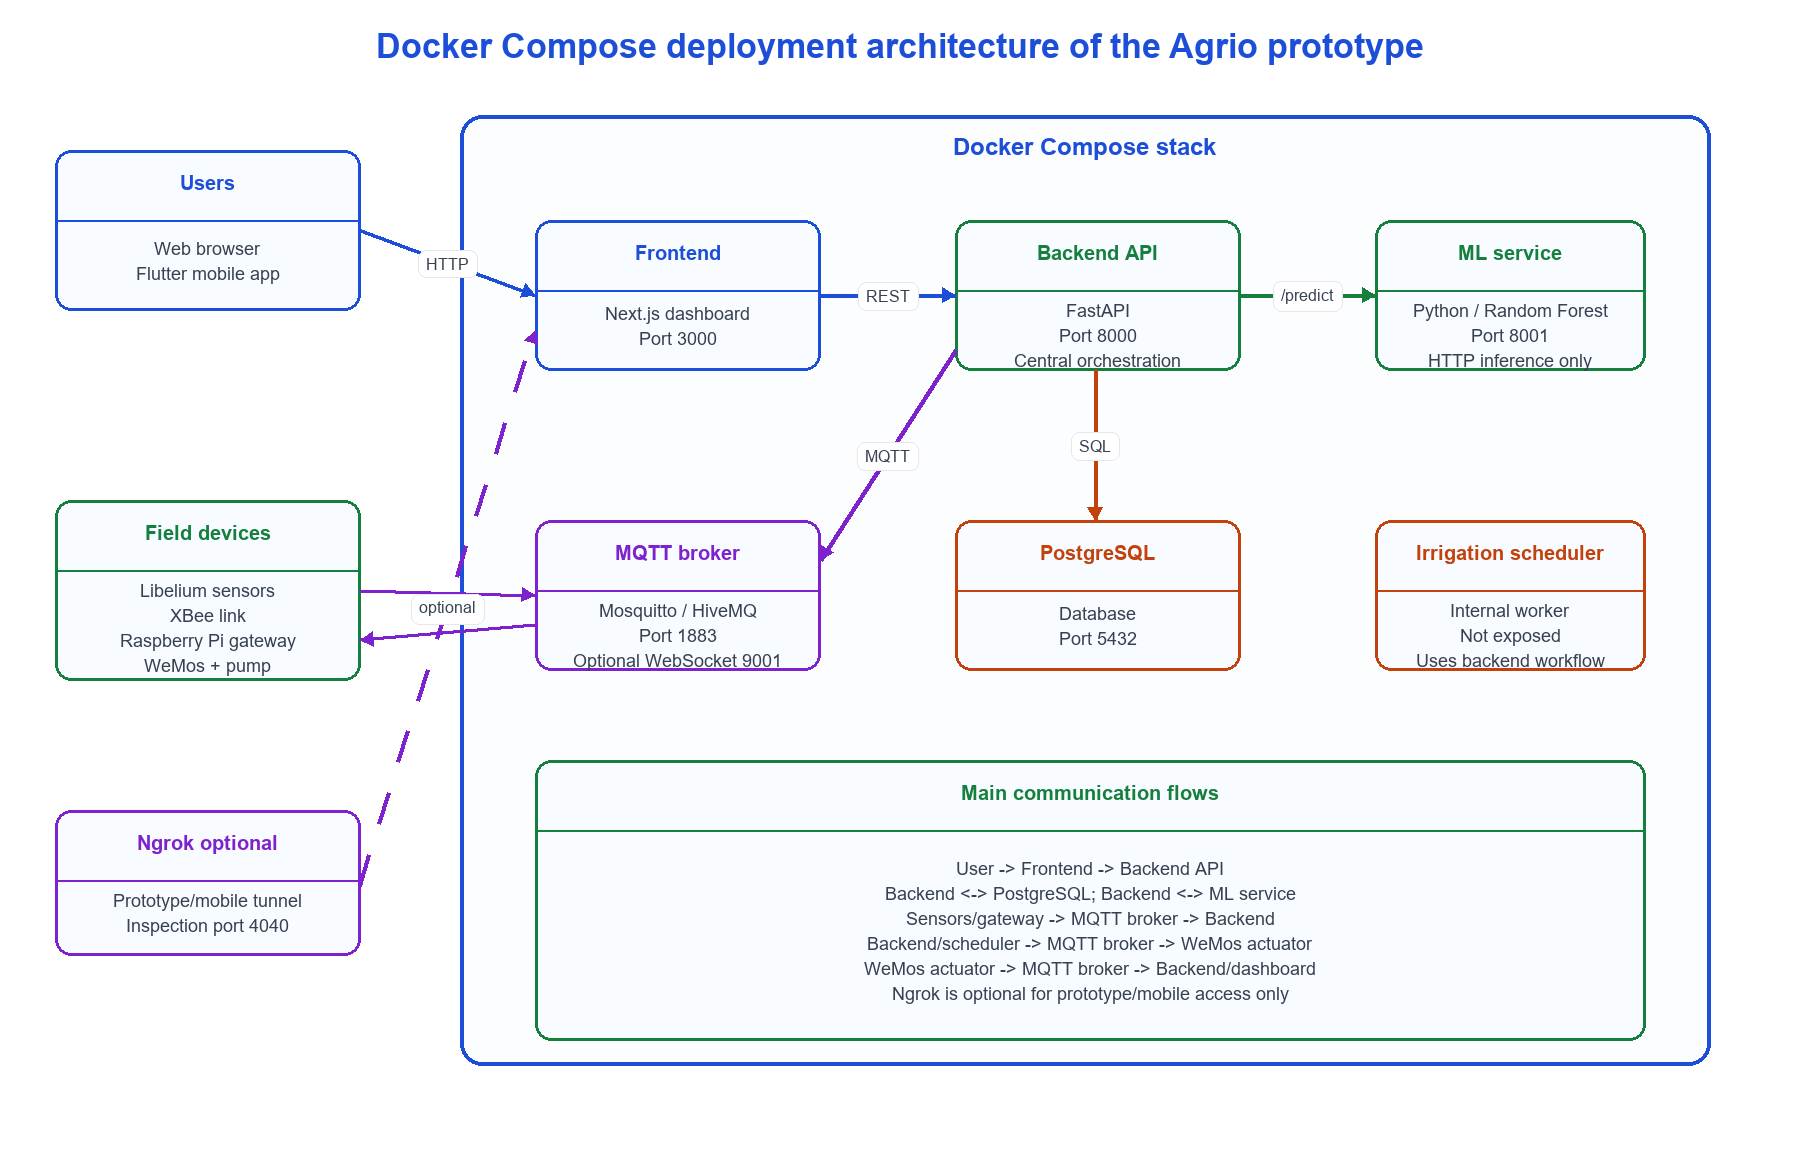
\includegraphics[width=0.95\textwidth,height=0.75\textheight,keepaspectratio]{figures/chapter_06/figure_5_6_deployment_architecture_corrected.png}
    \caption{Docker Compose service organization of the deployed Agrio platform.}
    \label{fig:10-1-docker-compose-service-organization-of-the-deployed-agrio-platfor}
\end{figure}

The running container evidence confirms that the prototype services are executed as a coordinated local deployment rather than as isolated scripts.

\begin{figure}[H]
    \centering
    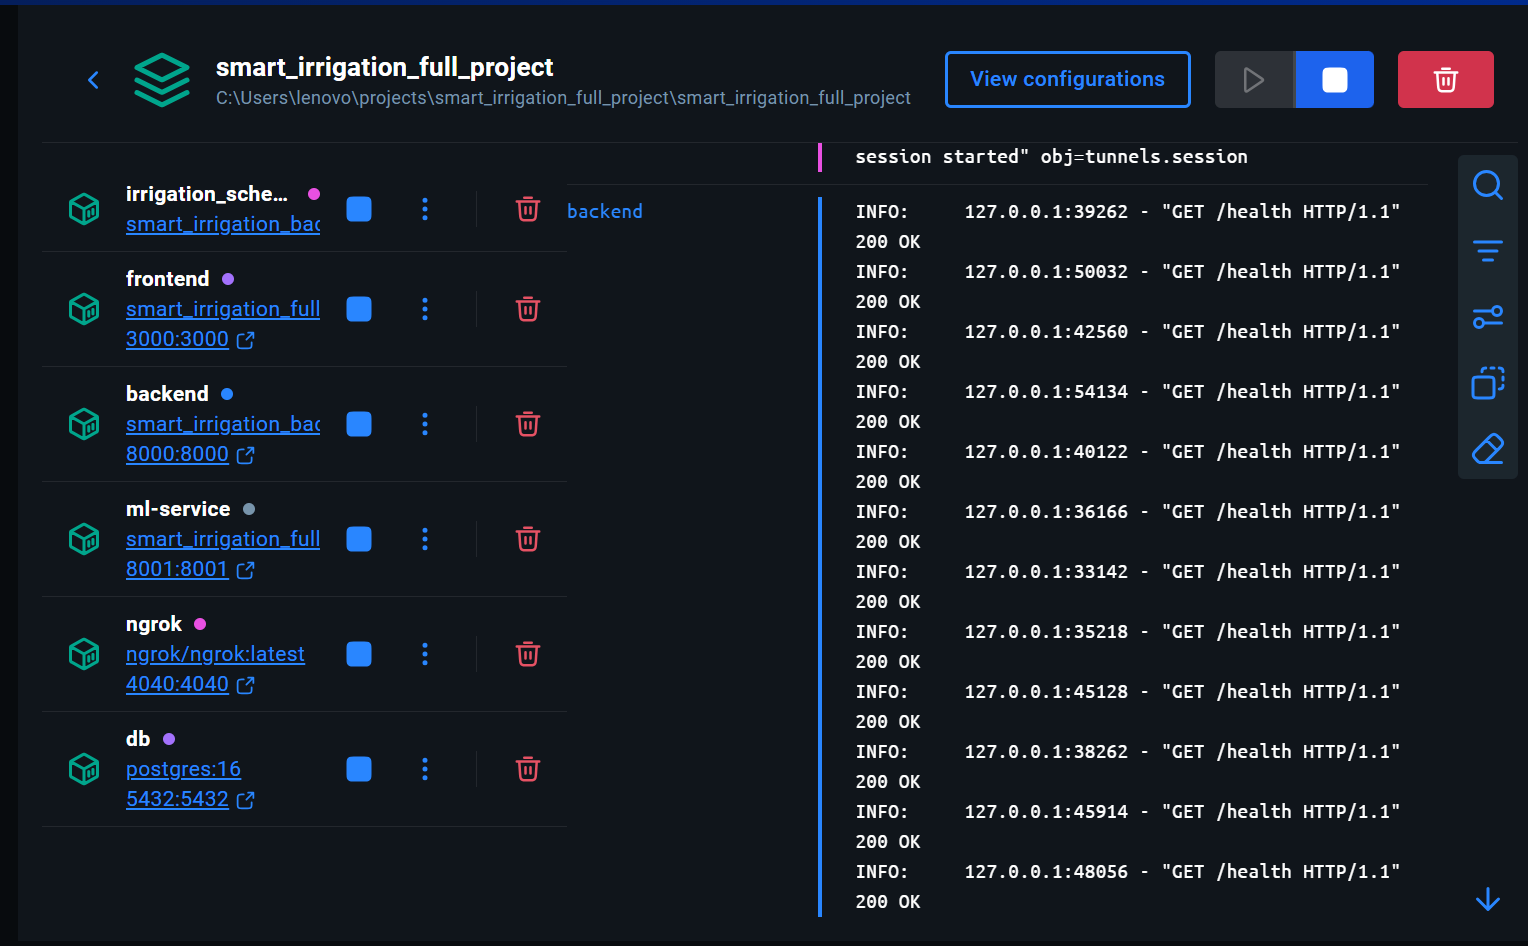
\includegraphics[width=0.9\textwidth,height=0.75\textheight,keepaspectratio]{figures/chapter_10/Figure 10.2 — Running Docker containers of the deployed Digital Twin smart irrigation platform.png}
    \caption{Running Docker containers of the deployed Digital Twin smart irrigation platform.}
    \label{fig:10-2-running-docker-containers-of-the-deployed-digital-twin-smart-irri}
\end{figure}

\section{Deployment communication flow}

Figure~\ref{fig:deployment_communication_flow} summarizes the runtime communication paths of the deployed Agrio prototype. The objective of this figure is not to repeat all Docker Compose configuration details, but to show how the main services exchange data during operation. Detailed port values, service roles, and operational evidence are documented separately in Table~\ref{tab:docker_compose_ports} and Table~\ref{tab:deployment_services_roles}.

The communication flow can be divided into four groups. First, users access the web dashboard or mobile interface, which communicates with the FastAPI backend through REST requests. Second, the backend reads and writes persistent data in PostgreSQL. Third, the backend sends feature payloads to the ML service over HTTP and receives prediction responses. Fourth, sensor telemetry, actuator commands, and WeMos status feedback are exchanged through MQTT topics.

\begin{figure}[H]
    \centering
    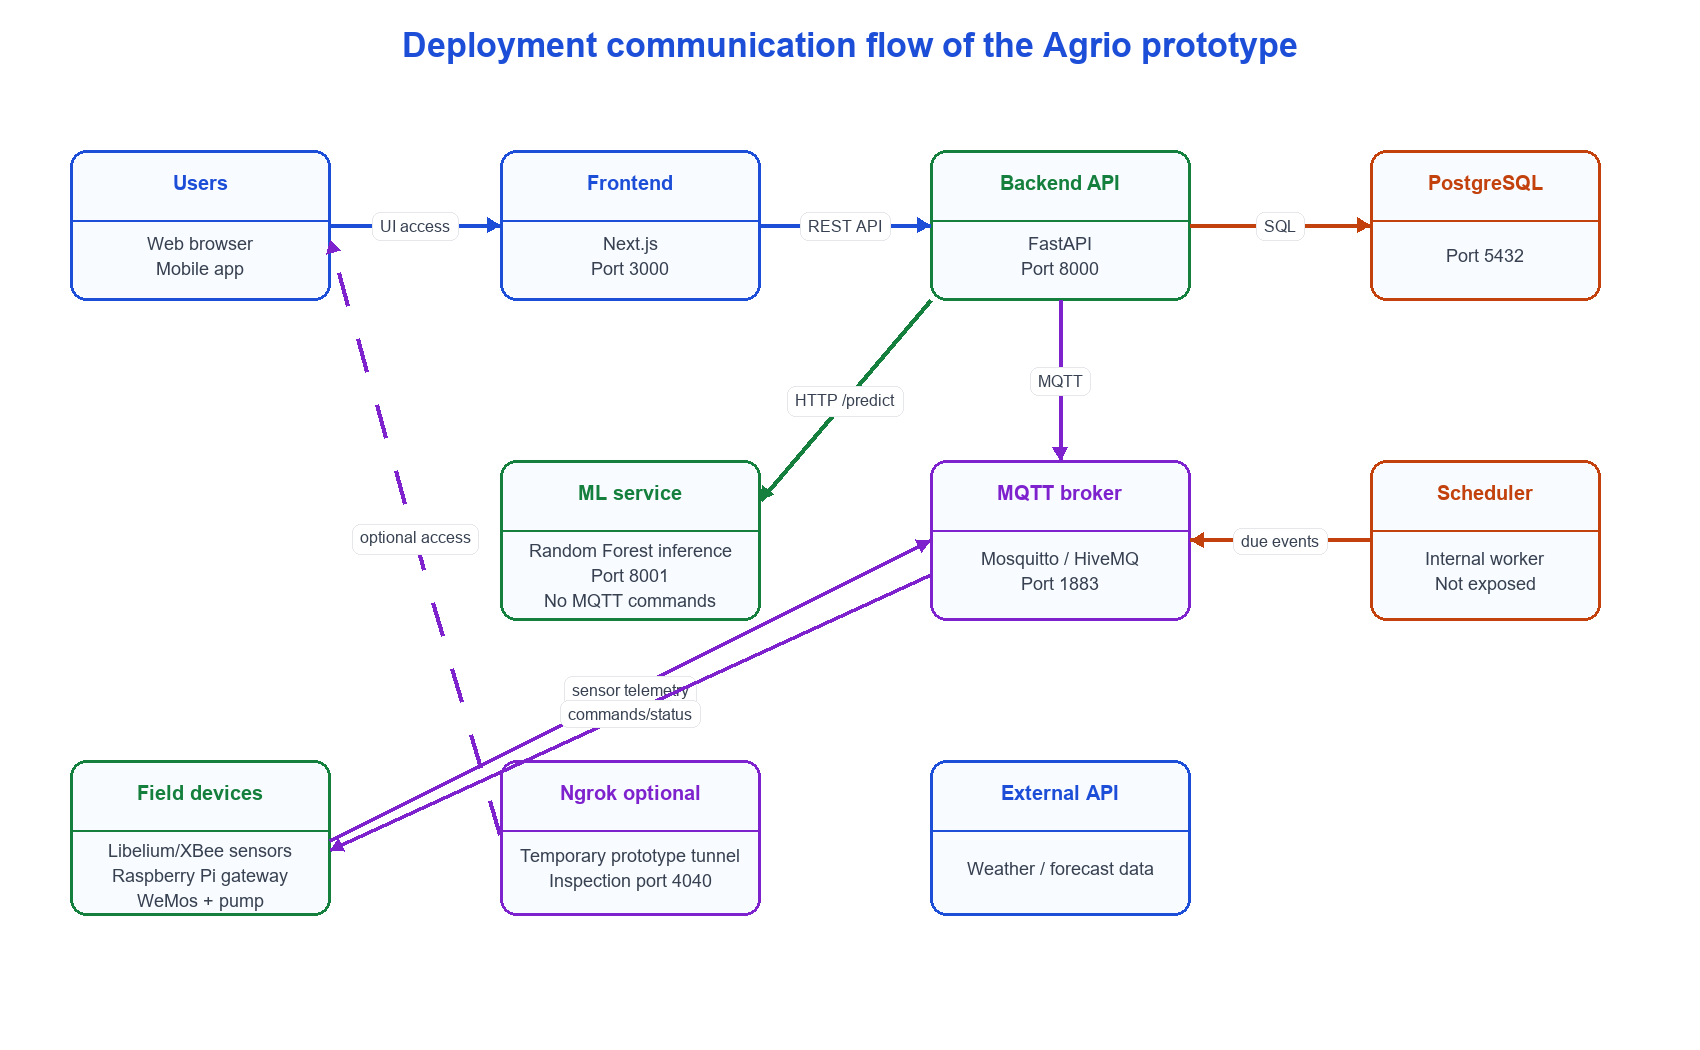
\includegraphics[width=0.95\textwidth,height=0.78\textheight,keepaspectratio]{figures/chapter_10/figure_10_3_deployment_communication_flow_corrected.png}
    \caption{Simplified deployment communication flow between frontend, backend, database, ML service, MQTT broker, scheduler, external API, and field devices.}
    \label{fig:deployment_communication_flow}
\end{figure}

The frontend service exposes the user-facing dashboard on port \texttt{3000}. It does not access the database or the MQTT broker directly. Instead, it retrieves monitoring data, Digital Twin states, predictions, recommendations, schedules, and actuator status through the backend API.

The backend service is the central orchestration point of the deployment. It exposes the FastAPI API on port \texttt{8000}, communicates with PostgreSQL through SQL queries, calls the ML service for inference, requests weather data from the external weather API, and publishes or consumes MQTT messages depending on the workflow.

The PostgreSQL service runs on port \texttt{5432} during local prototype validation. It stores the agricultural structure, sensor readings, weather records, Digital Twin states, prediction results, simulation outputs, recommendations, irrigation events, control commands, and execution feedback.

The ML service runs on port \texttt{8001}. It receives HTTP prediction requests from the backend and returns irrigation outputs such as \texttt{need\_irrigation}, \texttt{suggested\_hour}, confidence values, and recommended action. The ML service does not directly control the pump. Physical commands remain under backend and scheduler control.

The MQTT broker receives telemetry from sensors and actuator status messages from the WeMos controller. It also carries actuator commands published by the backend when the user validates a decision, manually triggers control, or when a scheduled irrigation event is executed. This separates asynchronous field communication from synchronous REST API communication.

The irrigation scheduler is represented as an internal worker. It checks scheduled irrigation events and triggers the documented command workflow when an event becomes due. It is not exposed as a public user-facing port in the prototype.

Ngrok is shown as an optional testing component. It provides a temporary public tunnel for mobile or external access during demonstrations, while its local inspection interface is available on port \texttt{4040}. It is not considered a production deployment mechanism.

\begin{table}[H]
\centering
\small
\caption{Main deployment communication flows.}
\label{tab:deployment_communication_flows}
\begin{tabular}{p{0.25\textwidth}p{0.30\textwidth}p{0.30\textwidth}}
\hline
\textbf{Flow} & \textbf{Direction} & \textbf{Purpose} \\
\hline
User access & User device $\rightarrow$ frontend & Access dashboard and mobile views. \\
REST API & Frontend/mobile $\rightarrow$ backend & Retrieve monitoring, prediction, simulation, schedule, and control data. \\
Database access & Backend $\leftrightarrow$ PostgreSQL & Persist and query Digital Twin lifecycle data. \\
ML inference & Backend $\leftrightarrow$ ML service & Send feature payloads and receive prediction outputs. \\
Weather request & Backend $\leftrightarrow$ Open-Meteo API & Retrieve weather and forecast information. \\
Sensor telemetry & Sensors/gateway $\rightarrow$ MQTT broker $\rightarrow$ backend & Transmit field measurements. \\
Actuator command & Backend/scheduler $\rightarrow$ MQTT broker $\rightarrow$ WeMos & Send pump or relay commands. \\
Status feedback & WeMos $\rightarrow$ MQTT broker $\rightarrow$ backend/dashboard & Report actuator status after commands. \\
Ngrok tunnel & External/mobile client $\rightarrow$ ngrok $\rightarrow$ local service & Provide temporary prototype access during testing. \\
\hline
\end{tabular}
\end{table}

\section{Service responsibilities}

The deployed prototype is divided into services with explicit responsibilities. PostgreSQL stores the \texttt{smart\_irrigation} schema and supports traceability from measurement to decision and feedback. The ML service loads Random Forest artifacts and exposes inference endpoints on port \texttt{8001}. The backend exposes the FastAPI API, orchestrates MQTT ingestion, calls the ML service, persists results, and publishes actuator commands. The frontend exposes the web dashboard on port \texttt{3000}. The scheduler runs as an internal worker and is not exposed as a public port. MQTT configuration connects backend ingestion and actuator workflows to the selected broker.

This organization keeps service boundaries clear. The frontend does not access PostgreSQL or MQTT directly. The ML service does not publish actuator commands. Physical commands remain under the backend and scheduler workflow, which publishes the documented WeMos commands through MQTT and records feedback.

\begin{footnotesize}
\setlength{\tabcolsep}{2pt}
\begin{longtable}{@{}>{\raggedright\arraybackslash}p{0.28\textwidth}>{\raggedright\arraybackslash}p{0.28\textwidth}>{\raggedright\arraybackslash}p{0.28\textwidth}@{}}
\caption{Deployment services and roles}
\label{tab:deployment_services_roles}\\
\toprule
Service & Role & Evidence to include \\
\midrule
\endfirsthead
\toprule
Service & Role & Evidence to include \\
\midrule
\endhead
postgres & Stores smart\_irrigation schema & Docker container and database screenshot \\
ml-service & Loads Random Forest models and predicts irrigation outputs & /health, /metadata, /predict screenshots \\
backend & API, MQTT ingestion, twin update, recommendations, commands & Health response, API response, and logs \\
frontend & Web dashboard and user workspaces & Dashboard screenshots \\
irrigation-scheduler & Internal worker that executes scheduled pump events & Scheduler logs or event status \\
ngrok & Mobile access tunnel used during prototype testing & Ngrok forwarding screenshot \\
MQTT configuration & Connects the backend and actuator workflow to the selected MQTT broker & Broker connection and topic evidence \\
\bottomrule
\end{longtable}
\end{footnotesize}

\section{Prototype mobile access with Ngrok}

Ngrok can expose local services for mobile testing, and its local inspection interface is available on port \texttt{4040}. This is useful when the Flutter application must access the backend from a mobile device during demonstrations.

\begin{figure}[H]
    \centering
    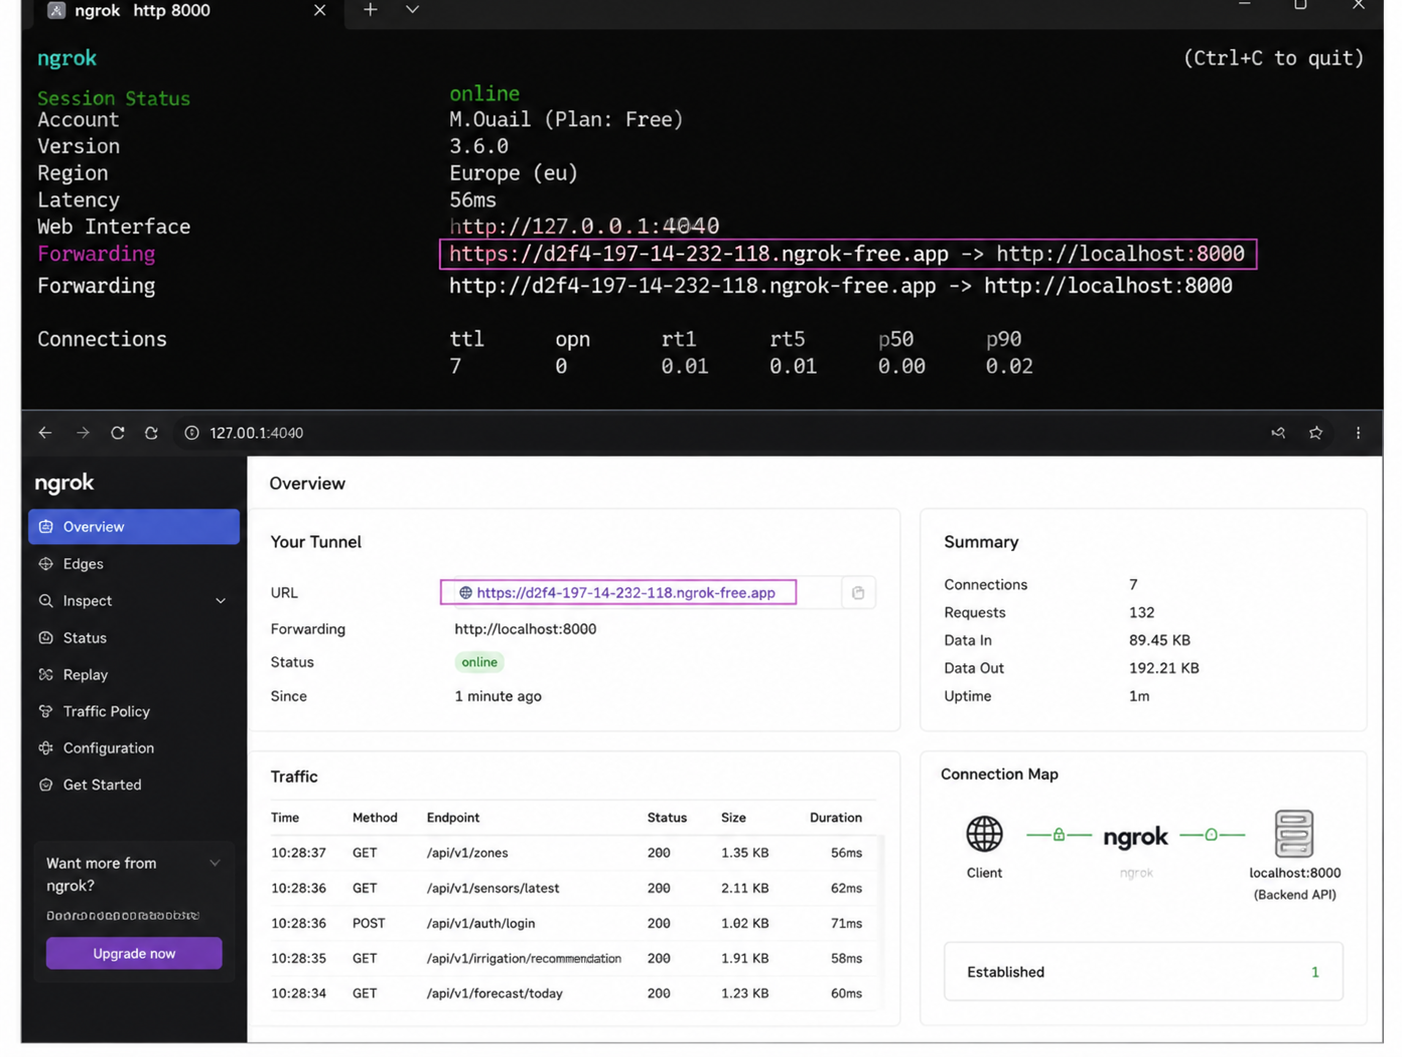
\includegraphics[width=0.9\textwidth,height=0.75\textheight,keepaspectratio]{figures/chapter_10/figure_10_4_ngrok_tunnel_clean.png}
    \caption{Ngrok tunnel used to expose local services for mobile access during prototype testing.}
    \label{fig:10-4-ngrok-tunnel-used-to-expose-local-services-for-mobile-access-duri}
\end{figure}

\section{Deployment limitations}

The deployment is suitable for prototype demonstration but not yet for production. A production environment would require HTTPS, secure credentials, role-based access control, backups, monitoring, and hardened MQTT authentication.

\section{Conclusion}

This chapter showed that Agrio is deployed as a reproducible multi-service prototype rather than as a single script or static dashboard. The deployment separates persistence, API orchestration, ML inference, frontend access, scheduling, MQTT communication, and mobile testing support. This separation makes the validation workflow easier to reproduce while also making clear that production deployment would still require stronger security, monitoring, backups, and operational hardening.
